\documentclass{scrartcl}
\usepackage{geometry}
\usepackage{csquotes}
\usepackage{hyperref}
\usepackage{graphicx}
\graphicspath{ {images/} }

\geometry{legalpaper, portrait, margin=1in}
 
\title{Harvard University, John A. Paulson School of Engineering and Applied Sciences \newline}
\subtitle{CS236r Project Update\\ Computational Results For Peer-Prediction and Crowdsourced Judgement Elicitation}
\author{Virgile Audi (vaudi@g.harvard.edu)\\
		Charles Liu (cliu02@g.harvard.edu)}

\begin{document}
 
\maketitle
	  
\section{Updates}
\subsection{Crowdsourced Elicitation}
A simple Python framework has been written to easily test different strategies for the agents. There is a base agent class with three functions: proficiency, has\_effort, and report each of which return a value $\in [0,1]$. Using the task assignment algorithm described in Section 5, we replicated the major results from the paper computationally, with proficiency $\geq 0.5$, has\_effort 0 and 1 for giving no effort and full effort respectively, and report 0 and 1 for reporting untruthfully and truthfully respectively.

Plots can be found in the Results section, including the result supporting Lemma 8 which we found most interesting: 
\begin{displayquote}
Suppose the probability of agent i using strategy (1, X) is $\delta$ and strategy $(0, r_i)$ is $1-\delta$ for each task $j \in J(i)$. Suppose i'’s potential reference raters $r_j (i)$ use strategies (1, X) and $(0, r_{r_j} (i))$ with probabilities $\epsilon_{r_j}(i)$ and $1-\epsilon_{r_j}(i)$ respectively, for each task $j \in J(i)$. If $\epsilon_{r_j}(i) > 0$ for any reference rater with proficiency $p_{r_j} (i) > \frac{1}{2}$, then agent i has a (strict) profitable deviation to $\delta'=1$, i.e., to always using strategy (1, X), for all values of $r_i \in [0,1]$
\end{displayquote}

The rewards in each scenario are scaled by 10 to see an interesting separation between strategies - as the paper states when presenting the reward formula, the scaling factor can be used to outweigh any costs incurred to the agent for completing a task. For the remainder of the project, how costs are related to effort will be the focus. In the paper their assumptiosn regarding cost are very general: they assume that costs are 0 for no effort and some constant value for full effort, though they note that all of their results apply when cost and proficiency are linearly scaled to effort. 

This is a very unrealistic assumption - as noted towards the end of the paper a natural extension would be to introduce the concept of difficulty to particular tasks. In this scenario proficiency on a task is a function of both effort and difficulty, and costs are a function of effort (perhaps convexly). It would seem the optimal strategy would then be to give little effort on difficult tasks and focus on getting rewards for the easier tasks. The first goal would be to validate this intuition. Finally, we would like to come up with a modification for the reward formula to incentivize giving effort to more difficult problems.


\section{Results}
\subsection{Crowdsourced Elicitation}
\begin{figure}
	\caption{Computational results of different equilibriums vs. other strategies}
	\centering
	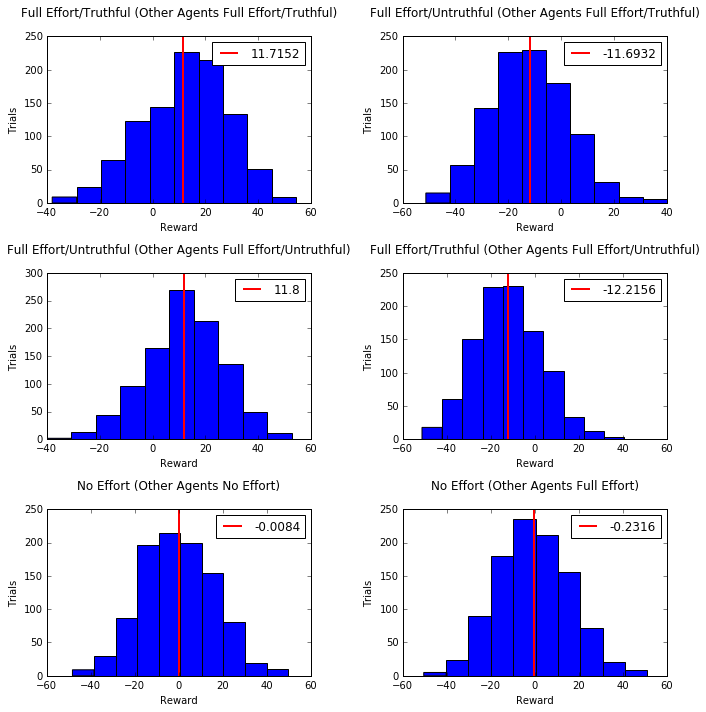
\includegraphics[width=1.0\textwidth]{cs_equilibriums}
\end{figure}
\begin{figure}
	\caption{Computational results of Lemma 8}
	\centering
	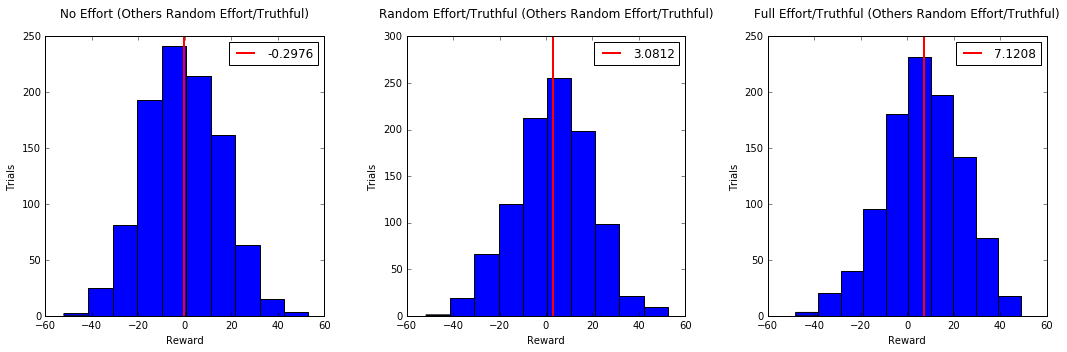
\includegraphics[width=1.0\textwidth]{cs_lemma8}
\end{figure}

\end{document}